%%%%%%%%%%%%%%%%%%%%%%%%%%%%%%%%%%%%%%%%%
% University/School Laboratory Report
% LaTeX Template
% Version 3.1 (25/3/14)
%
% This template has been downloaded from:
% http://www.LaTeXTemplates.com
%
% Original author:
% Linux and Unix Users Group at Virginia Tech Wiki 
% (https://vtluug.org/wiki/Example_LaTeX_chem_lab_report)
%
% License:
% CC BY-NC-SA 3.0 (http://creativecommons.org/licenses/by-nc-sa/3.0/)
%
%%%%%%%%%%%%%%%%%%%%%%%%%%%%%%%%%%%%%%%%%

%----------------------------------------------------------------------------------------
%	PACKAGES AND DOCUMENT CONFIGURATIONS
%----------------------------------------------------------------------------------------

%\documentclass{article}
\documentclass[a4paper,11pt]{exam}


\usepackage[version=3]{mhchem} % Package for chemical equation typesetting
\usepackage{siunitx} % Provides the \SI{}{} and \si{} command for typesetting SI units
\usepackage{graphicx} % Required for the inclusion of images
\usepackage{natbib} % Required to change bibliography style to APA
\usepackage{amsmath} % Required for some math elements 
\usepackage{listings}

\printanswers
\setlength\parindent{0pt} % Removes all indentation from paragraphs

\renewcommand{\labelenumi}{\alph{enumi}.} % Make numbering in the enumerate environment by letter rather than number (e.g. section 6)

\usepackage{titlesec}


%\usepackage{times} % Uncomment to use the Times New Roman font

%----------------------------------------------------------------------------------------
%	DOCUMENT INFORMATION
%----------------------------------------------------------------------------------------

\title{TP1: Spectral Clustering \\ Graphs in ML} % Title
\author{Thomas \textsc{Opsomer}} % Author name

\date{\today} % Date for the report

\begin{document}

\maketitle % Insert the title, author and date

%\begin{center}
%\begin{tabular}{l r}
%Date Performed: & January 1, 2012 \\ % Date the experiment was performed
%Partners: & James Smith \\ % Partner names
%& Mary Smith \\
%Instructor: & Professor Smith % Instructor/supervisor
%\end{tabular}
%\end{center}

% If you wish to include an abstract, uncomment the lines below
% \begin{abstract}
% Abstract text
% \end{abstract}

%----------------------------------------------------------------------------------------
%	1. Graph construction
%----------------------------------------------------------------------------------------

\section{Graph construction}

\begin{questions}
 
\question What is the purpose of the option parameter in worst\_case\_blob ?
\begin{solution}

The option in worst\_case\_blob aims at producing a dataset with a singularity: a point that is very far from all other points. To do this the functions creates a dataset generated according to a gaussian distribution ($randn$) but then the fonction csutomize the last element.
Each of its component is equal to the max of this component among all other points plus an additional parameter wihich is the option parameter. Consequently if we make this parameter big enough, the last datapoint has a very big norm compared to others, then it is very far from every other points (singularity/outlier).
\end{solution}

\question What happens when you change the generating parameter of worst\_case\_blob.m? What if the parameter is very large?

\begin{figure}[!h]
\begin{center}
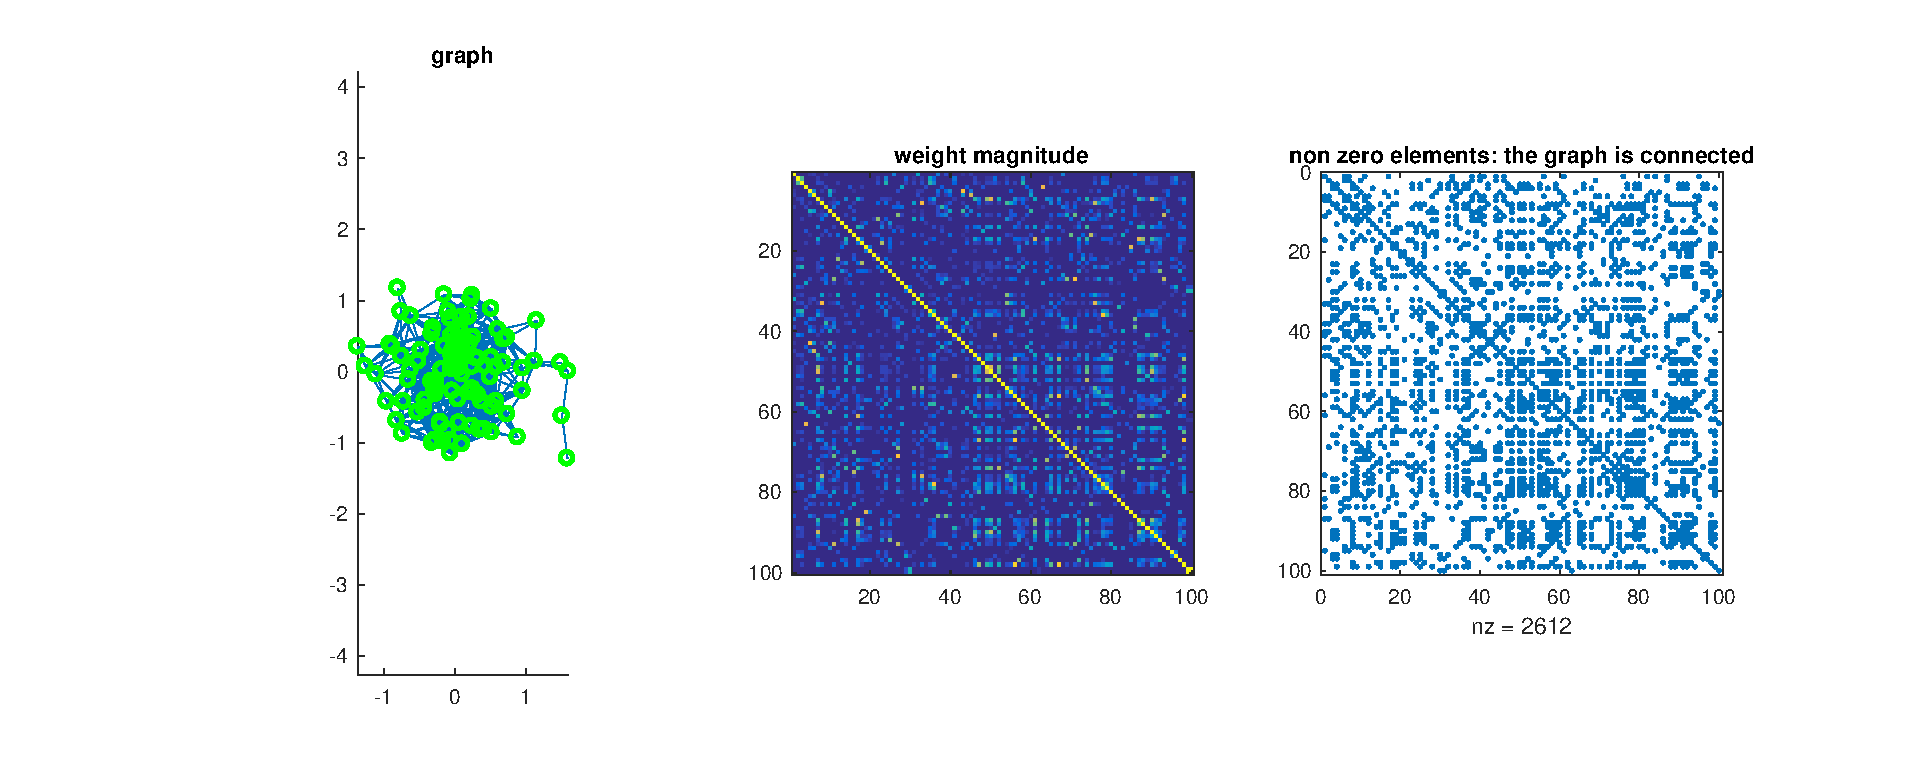
\includegraphics[width=13cm]{figures/word_case_0_01.eps}
\caption{$\epsilon$ graph for the worst case blob with parameter 0.01}
\label{word_case_0_01}
\end{center}
\end{figure}

\begin{figure}[!h]
\begin{center}
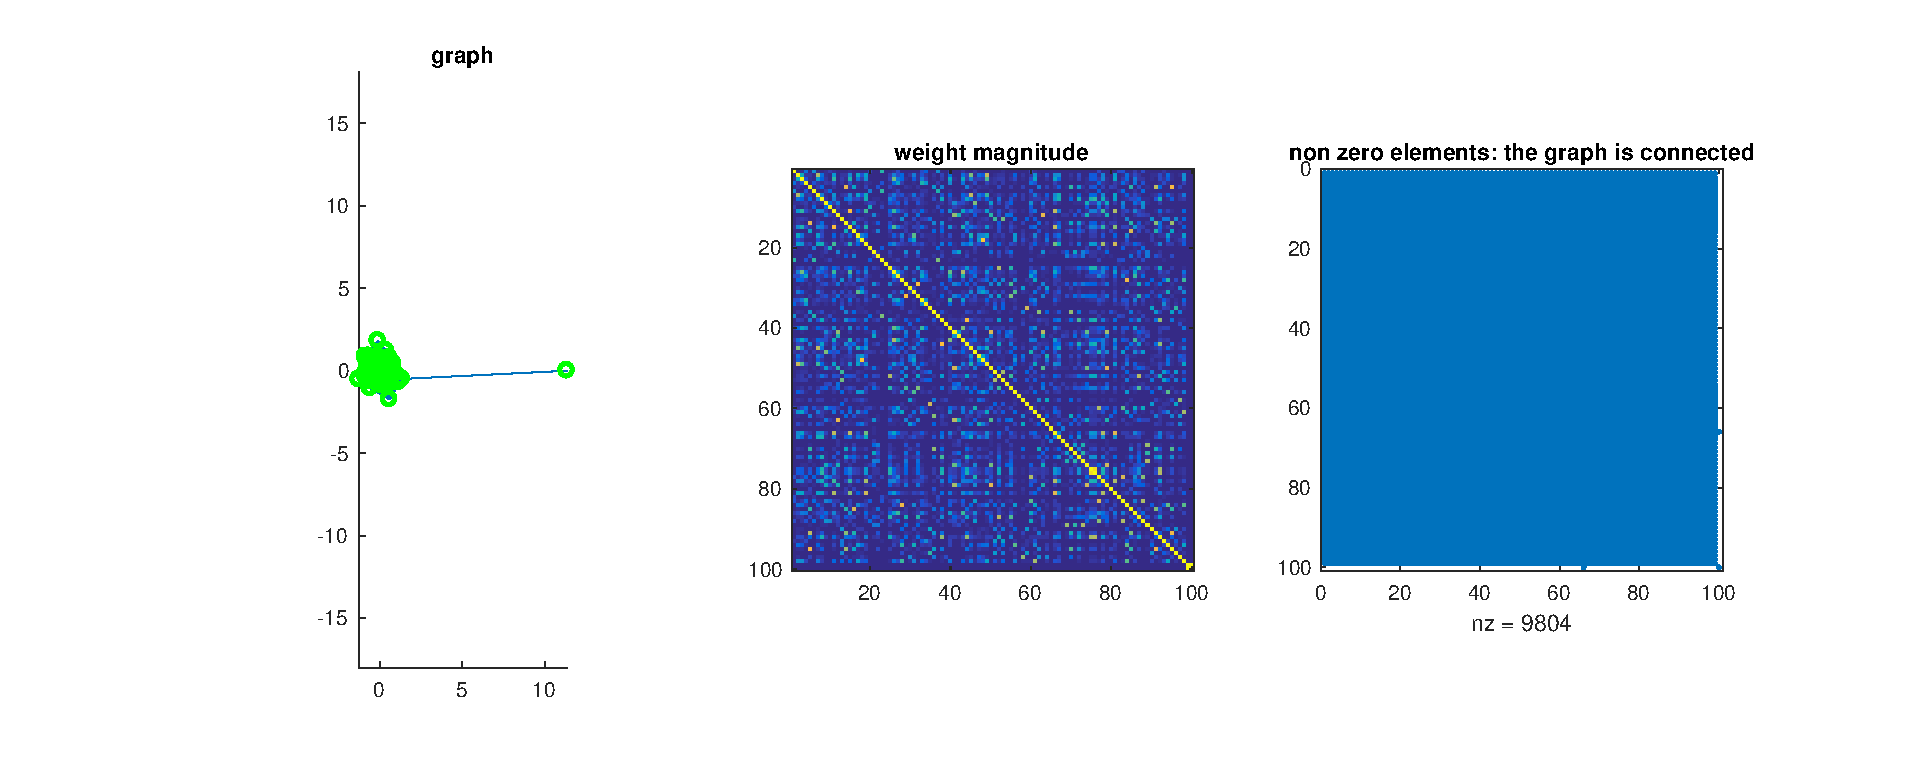
\includegraphics[width=13cm]{figures/word_case_10.eps}
\caption{$\epsilon$ graph for the worst case blob with parameter 10}
\label{word_case_10}
\end{center}
\end{figure}


\begin{solution}
Figure \ref{word_case_0_01} shows the $\epsilon$ graph with a generating parameter of 0.01 and figure \ref{word_case_10} shows the $\epsilon$ graph for a parameter of value 10. For each value the graph is connected because we choose $\epsilon$ for that. However the bigger the parameter get the farther gets the last points of the samples. Consequently the epsilon chosen is getting lower and lower and as a result the last point is connected to only a few points (and only one point when the parameter is big enough) but all other points are connected with each other because $\epsilon$ is very small. Look at the non-zero-element matrix of figure \ref{word_case_10}, all value are non zero except the last column and last row, representing the connection of the last points of the dataset. Here we see that the last points is only connected to 2 other points.


\end{solution}

\question Compare $k-nn$ to ? graphs. When is it easier to build a connected graph using $k-nn$?
\begin{solution}
While experimenting on building graph on the two\_moon and the blob dataset, it appear that $k-nn$ and $\epsilon$ graph behave very differently. When there are different scale in term of vertices distance It is easier to build a connected graph using $k-nn$. For instance on the two moon blob dataset, points are quite dispersed with some dense region and some more desert area. It is easy to build a connected graph using $k-nn$  with a few neighbors however if you try to build an $\epsilon$ graph you will have trouble trying to keep a region not too dense and another one connected.
Consequently when distances between data points have different scale among space regions, we would better use $k-nn$ and in other case try $\epsilon$-graph using the minimal spanning tree method to find $\epsilon$

\end{solution}
\end{questions}
 
%----------------------------------------------------------------------------------------
%	2. Spectral Clustering
%----------------------------------------------------------------------------------------

\section{Spectral Clustering}

\begin{questions}

\question Build a graph starting from the data loaded in two\_blobs\_clustering.m, and remember to keep the graph connected. Motivate your choice on which eigenvectors to use and how you computed the clustering assignments from the eigenvectors. Now compute a similar clustering using the builtin k-means and compare the results.

\begin{solution}
We used an $\epsilon$ graph with epsilon chosen as the minimum weight of the maximum spanning tree in order to have $\epsilon$ allowing the 2 blob to be connected. See figure \ref{2_1_1_eps_graph} for a graph representation of the two\_blob data. \\

As the graph is connected, the first eigenvalue is 0, and the first eigenvector is enough to split the dataset in the two clusters. As suggested in the course, I used Kmeans with 2 classes on the eigenvector coordinate and then assign cluster membership according to each points first eigenvector coordinate. As shown on figure \ref{two_blob_clustering}, both methods spectral clustering and k-means work very well.
\end{solution}

\begin{figure}[!h]
\begin{center}
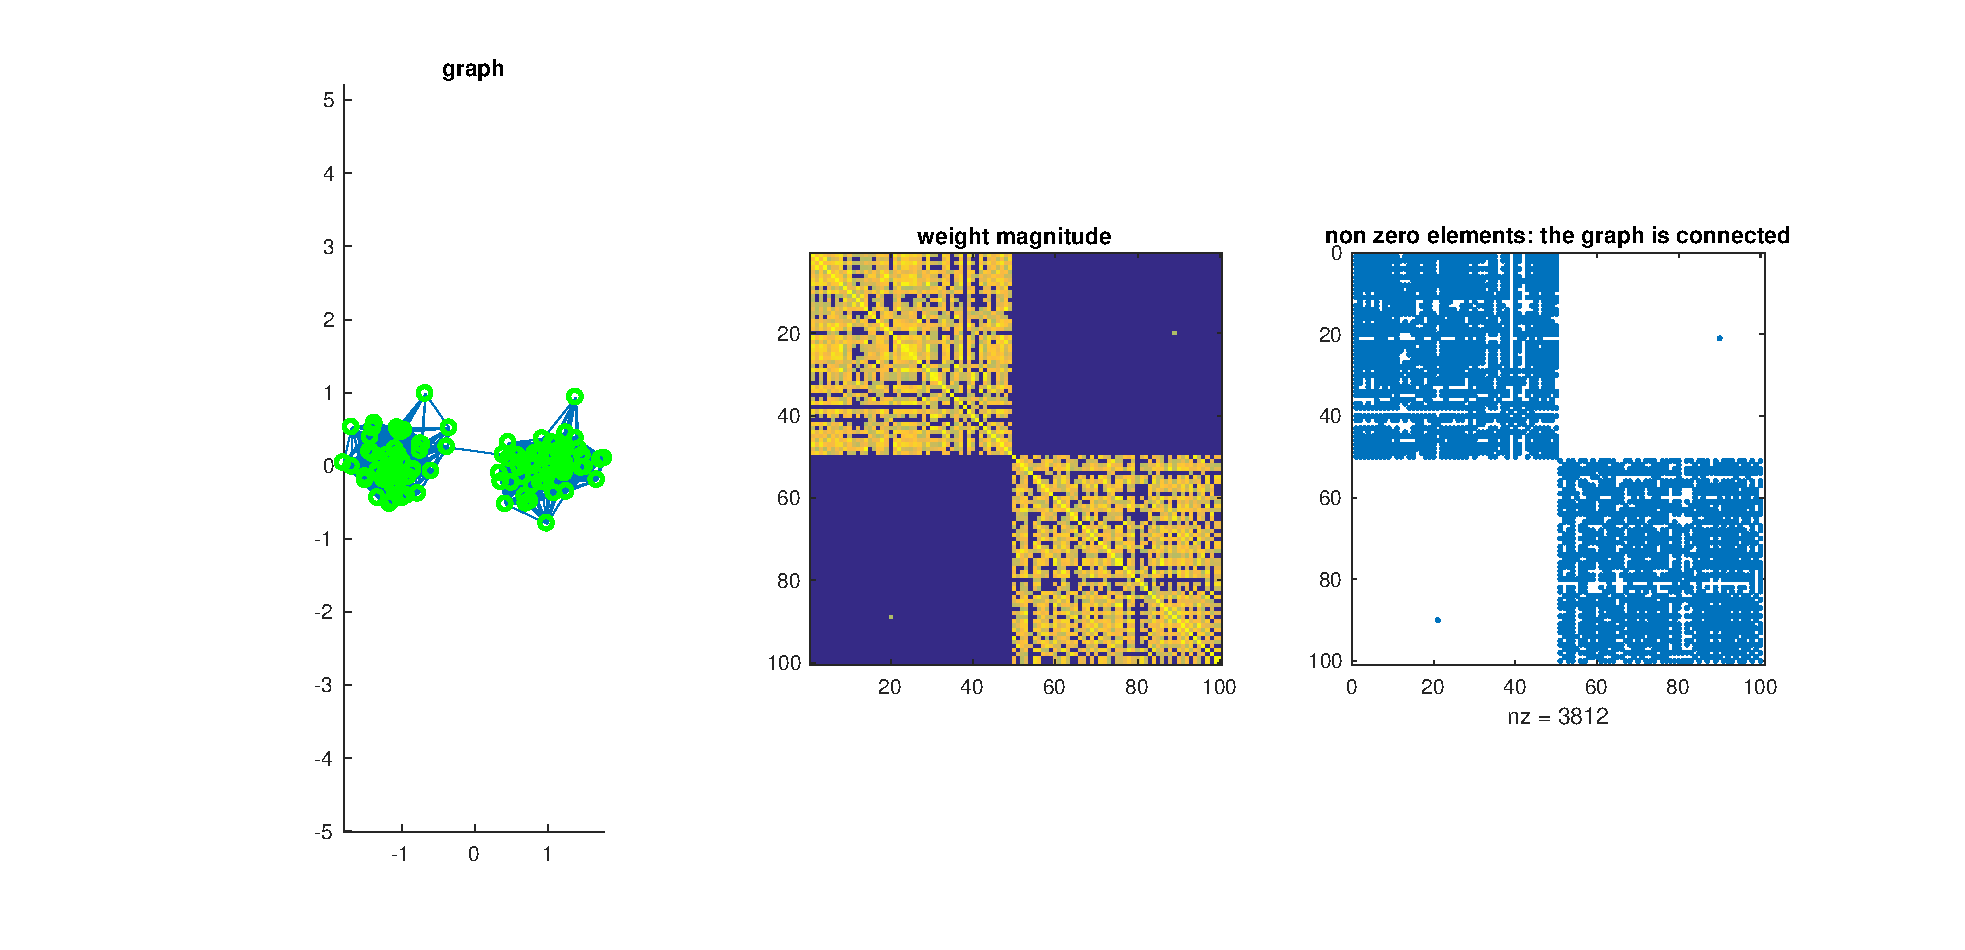
\includegraphics[width=13cm]{figures/2_1_1_eps_graph.eps}
\caption{$\epsilon$ graph for the two\_blob data, $\epsilon$ = 0.6784}
\label{2_1_1_eps_graph}
\end{center}
\end{figure}

\begin{figure}[!h]
\begin{center}
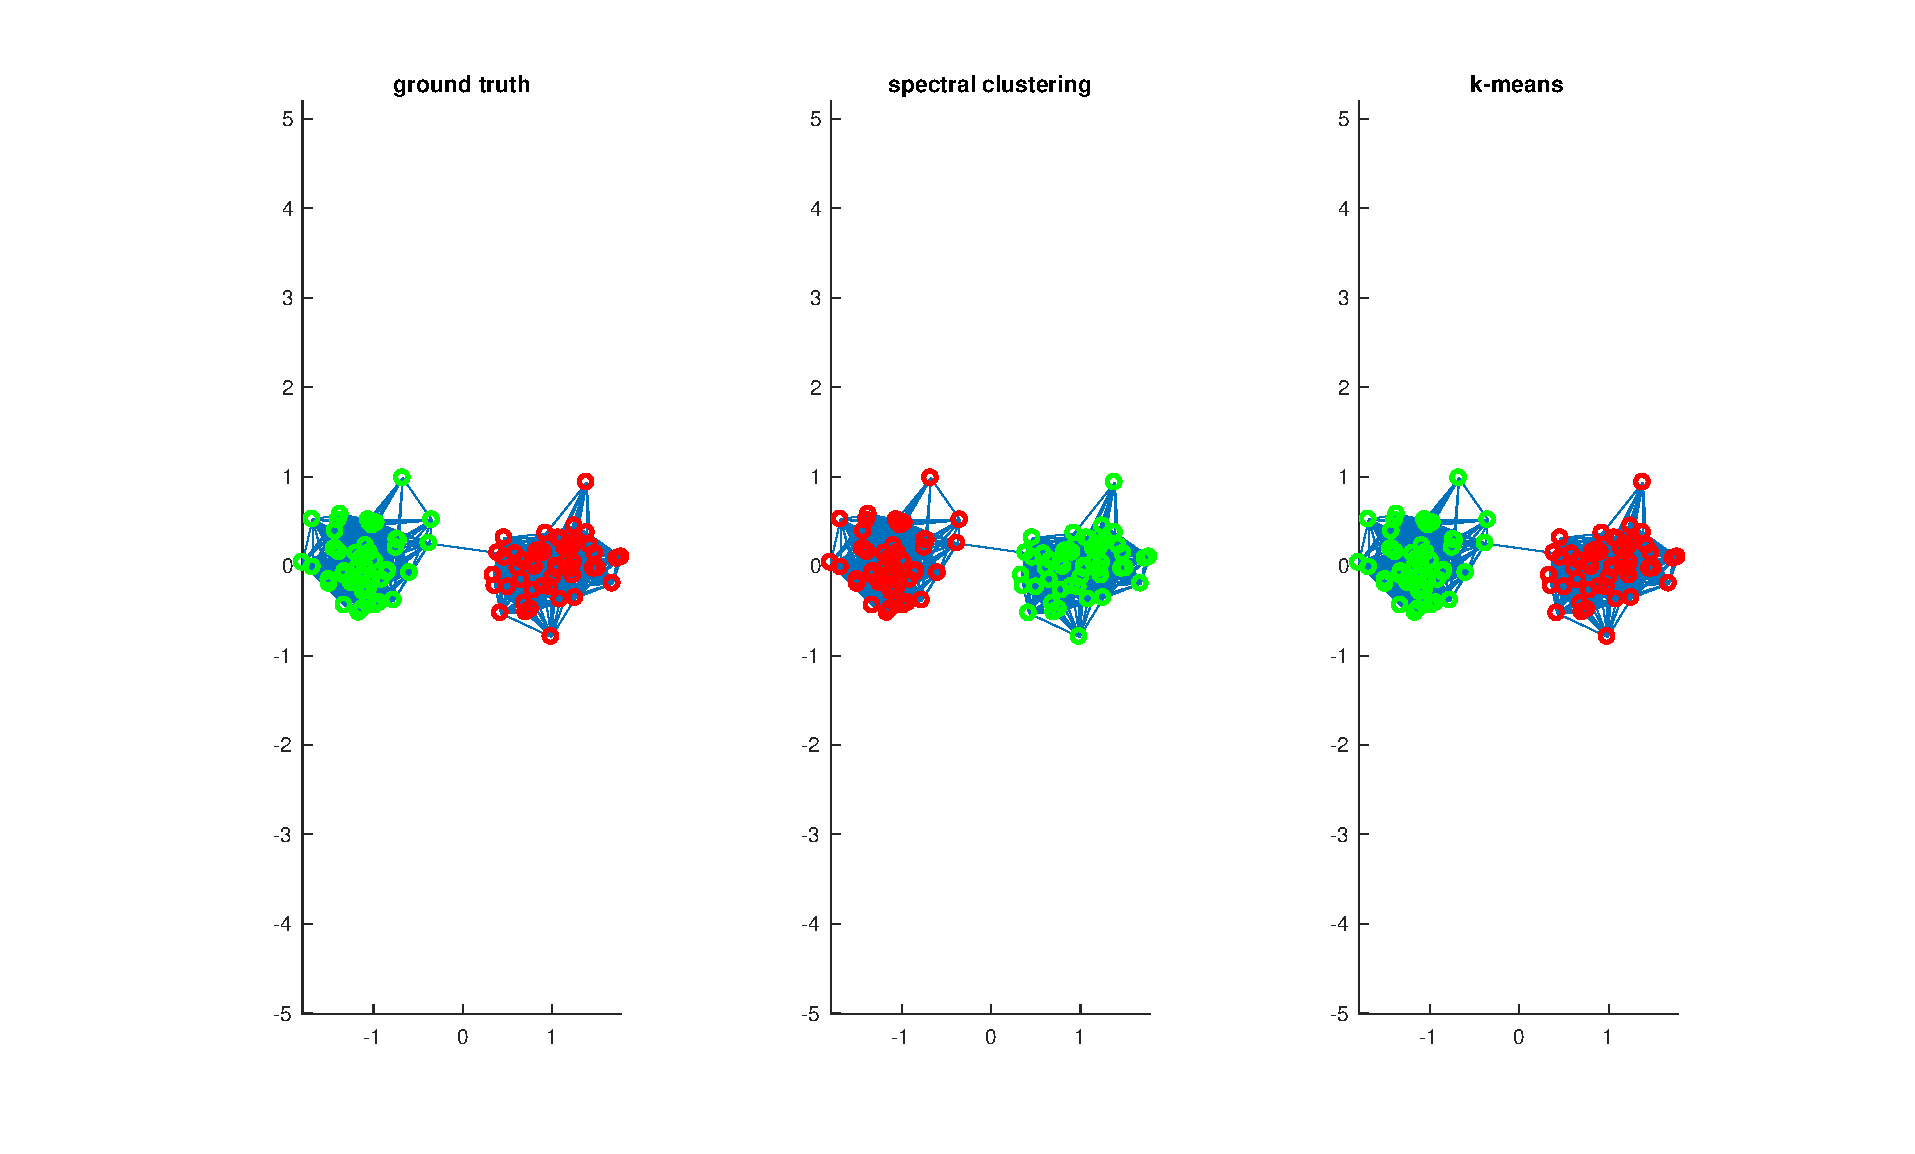
\includegraphics[width=13cm]{figures/two_blob_clustering.eps}
\caption{Results of two\_blob clustering.}
\label{two_blob_clustering}
\end{center}
\end{figure}


\question Build a graph starting from the data loaded in two\_blobs\_clustering. m, but this time makes it so that the two components are separate. How do you choose which eigenvectors to use in this case? Motivate your answer.

\begin{solution}
We used an $\epsilon$ graph with an $\epsilon$ a bit higher than before (0.7) to allow the two blob not to be connected. 
As the graph is no more connected but has two connected components, the eigenvalue 0 has multiplicity of 2, and we need to two first eigenvectors to bring enough information for clustering the dataset. Once again results for kmeans and spectral clustering are good.
\end{solution}

\question Look at find\_the\_bend.m. Generate a dataset with 4 blobs. Build a graph out of it and plot the first 15 eigenvalues of the Laplacian. Complete choose\_eig\_function.m to automatically choose the number of eigenvectors to include. The decision rule must adapt to the actual eigenvalues of the problem.

\begin{solution}

Looking at the plot of eigenvalue, for instance see figure \ref{15_eigenvalues}, we guess that we have to find the last index before a 'significant' increase in eigenvalue, more over we are looking at the first "significant" increase in eigenvalue.
Consequently I build the function choose\_eig\_function in two steps :
\begin{lstlisting}
function [eig_ind] = choose_eig_function(eigenvalues)
\end{lstlisting}

\begin{enumerate}
\item We find the index of the biggest increase in the eigenvalue function

\begin{lstlisting}
n_eig = size(eigenvalues,1);
discrete_derive = zeros(1, n_eig -1);
for i = 1:(n_eig -1)
    discrete_derive(i) = eigenvalues(i+1) - eigenvalues(i);
end
[~, m_index] = max(discrete_derive);
\end{lstlisting} 

\item Then find the first significant bump in increment looking at second derivative sign
\begin{lstlisting}
if m_index > 2
    % initialize
    best_m_index = m_index;
    % compute second derivative & look for the first sign
    % changes in second derivative
    descrete_derive_2 = zeros(1, m_index-1);
    for i = 1:(m_index-1)
        descrete_derive_2(i) = \
            discrete_derive(i+1) - discrete_derive(i);
        if descrete_derive_2(i) < 0
           && descrete_derive_2(i-1) > 0
            best_m_index = i;
            break
        end
    end
else
    best_m_index = m_index;
end
\end{lstlisting} 
\end{enumerate}

It works great in our case, answering a number of 4 eigenvectors to keep for the 4 blobs dataset.

\end{solution}


\begin{figure}[!h]
\begin{center}
\includegraphics[width=11cm]{figures/15_eigenvalues_bis.eps}
\caption{First 15 eigenvalues of a 4 blob dataset.}
\label{15_eigenvalues}
\end{center}
\end{figure}

\question Now increase the variance of the Blobs to $\sigma$2 = 0.20 as you keep plot- ting the eigenvalues. Use choose\_eig\_function.m. Do you see any difference?

\begin{solution}
Increasing $\sigma$ to 0.20 make the dataset much more complicated to cluster. If we apply directly the same process we used for $\sigma$=0.03 the clustering doesn't work well anymore. The data has much more variance so we need to refine the $\epsilon$ for the $\epsilon-graph$.  Actually I didn't manage to make it work with an $\epsilon$ graph, each times eigenvalues were not easy to separate with our choose\_eig\_function. Consequently I decided to use a $knn-graph$ for this case and results are much better. Which rejoins the discussion of question 1.3 about when using knn and $\epsilon$. Indeed now the dataset is less concentrated, many scale appear in the distance between vertices due to the high variance of each blob.
Our function choose\_eig\_function still word correctly, and returns the first four eigenvalues. See figure \ref{two_blob_knn_0_20} for results.
 
\end{solution}

\begin{figure}[!h]
\begin{center}
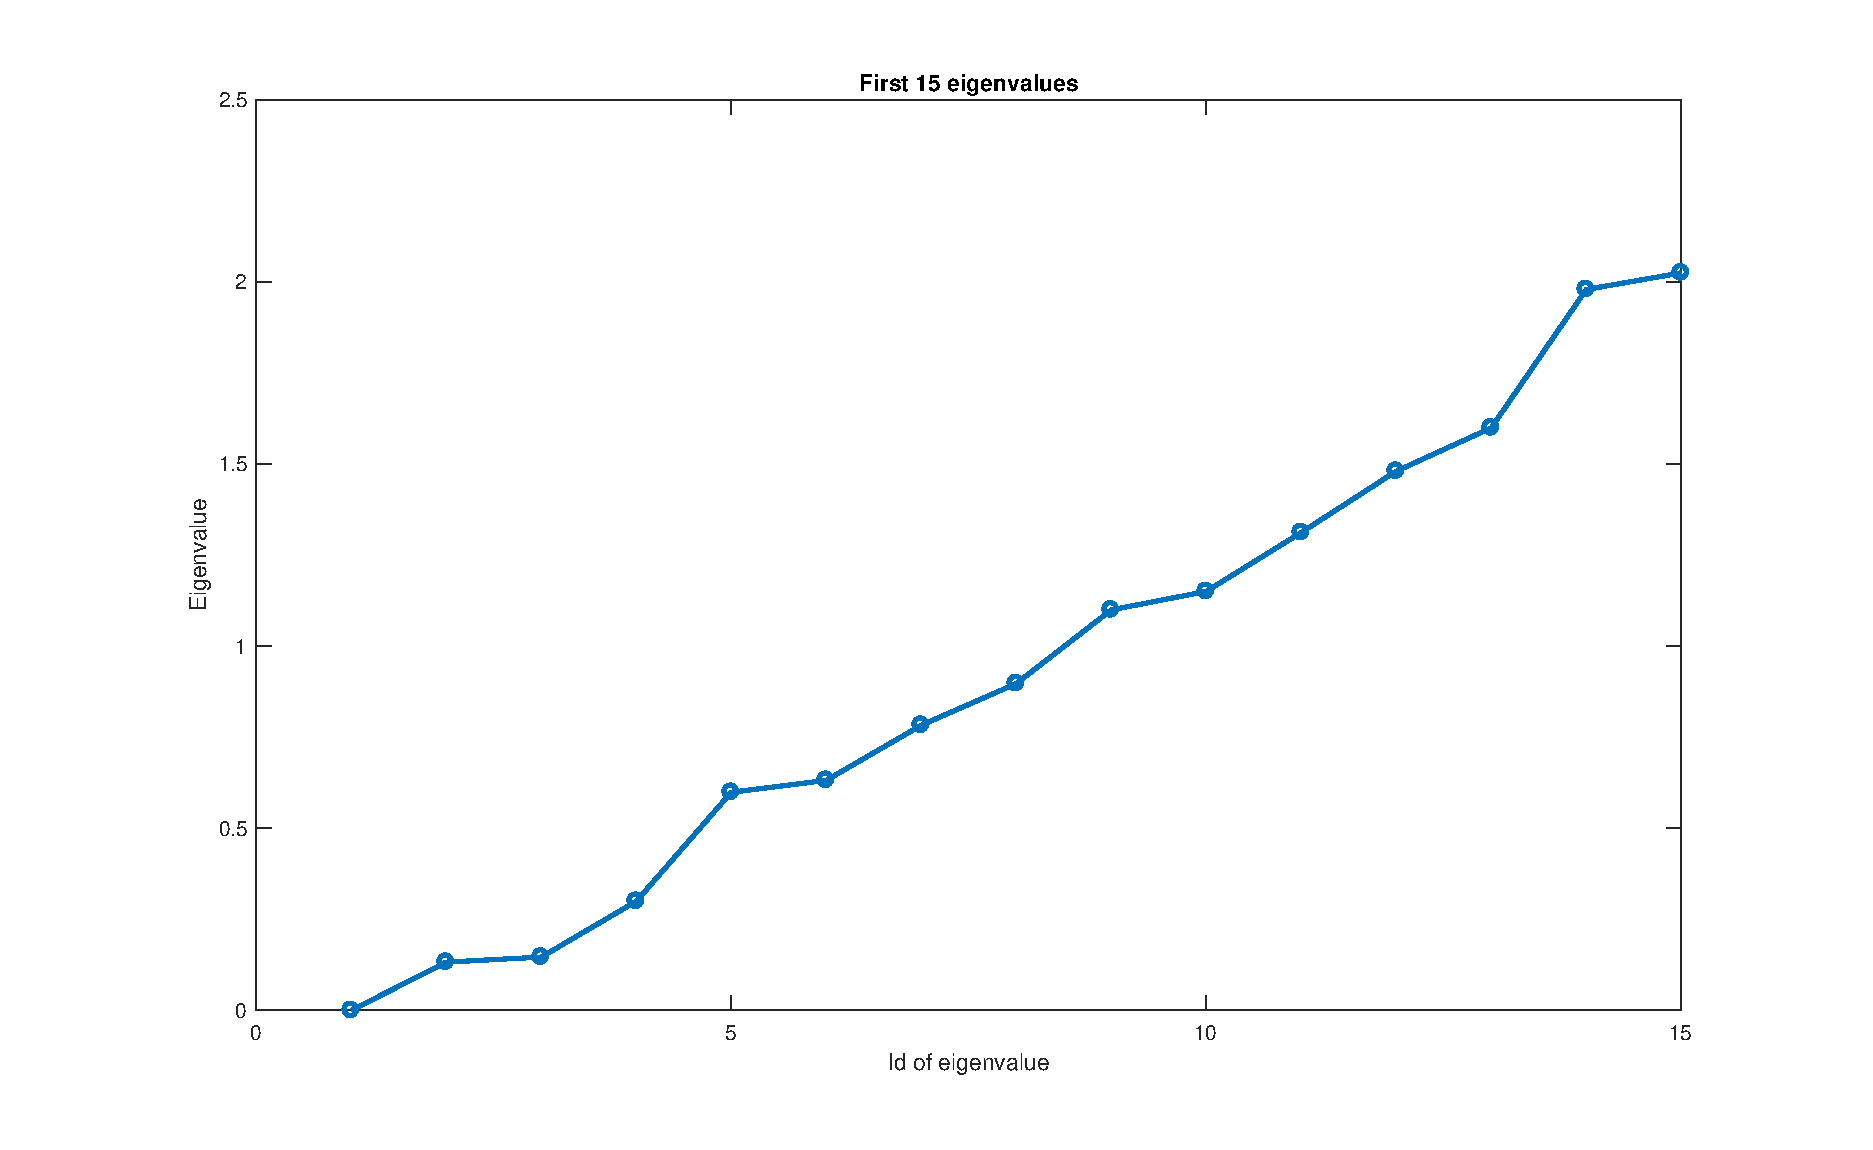
\includegraphics[width=13cm]{figures/15_eigen_4_blob_sigma_02_bis.eps}
\caption{First 15 eigenvalues of a 4 blob dataset with $\sigma$ = 0.20.}
\label{15_eigen_4_blob_sigma_02.eps}
\end{center}
\end{figure}

\begin{figure}[!h]
\begin{center}
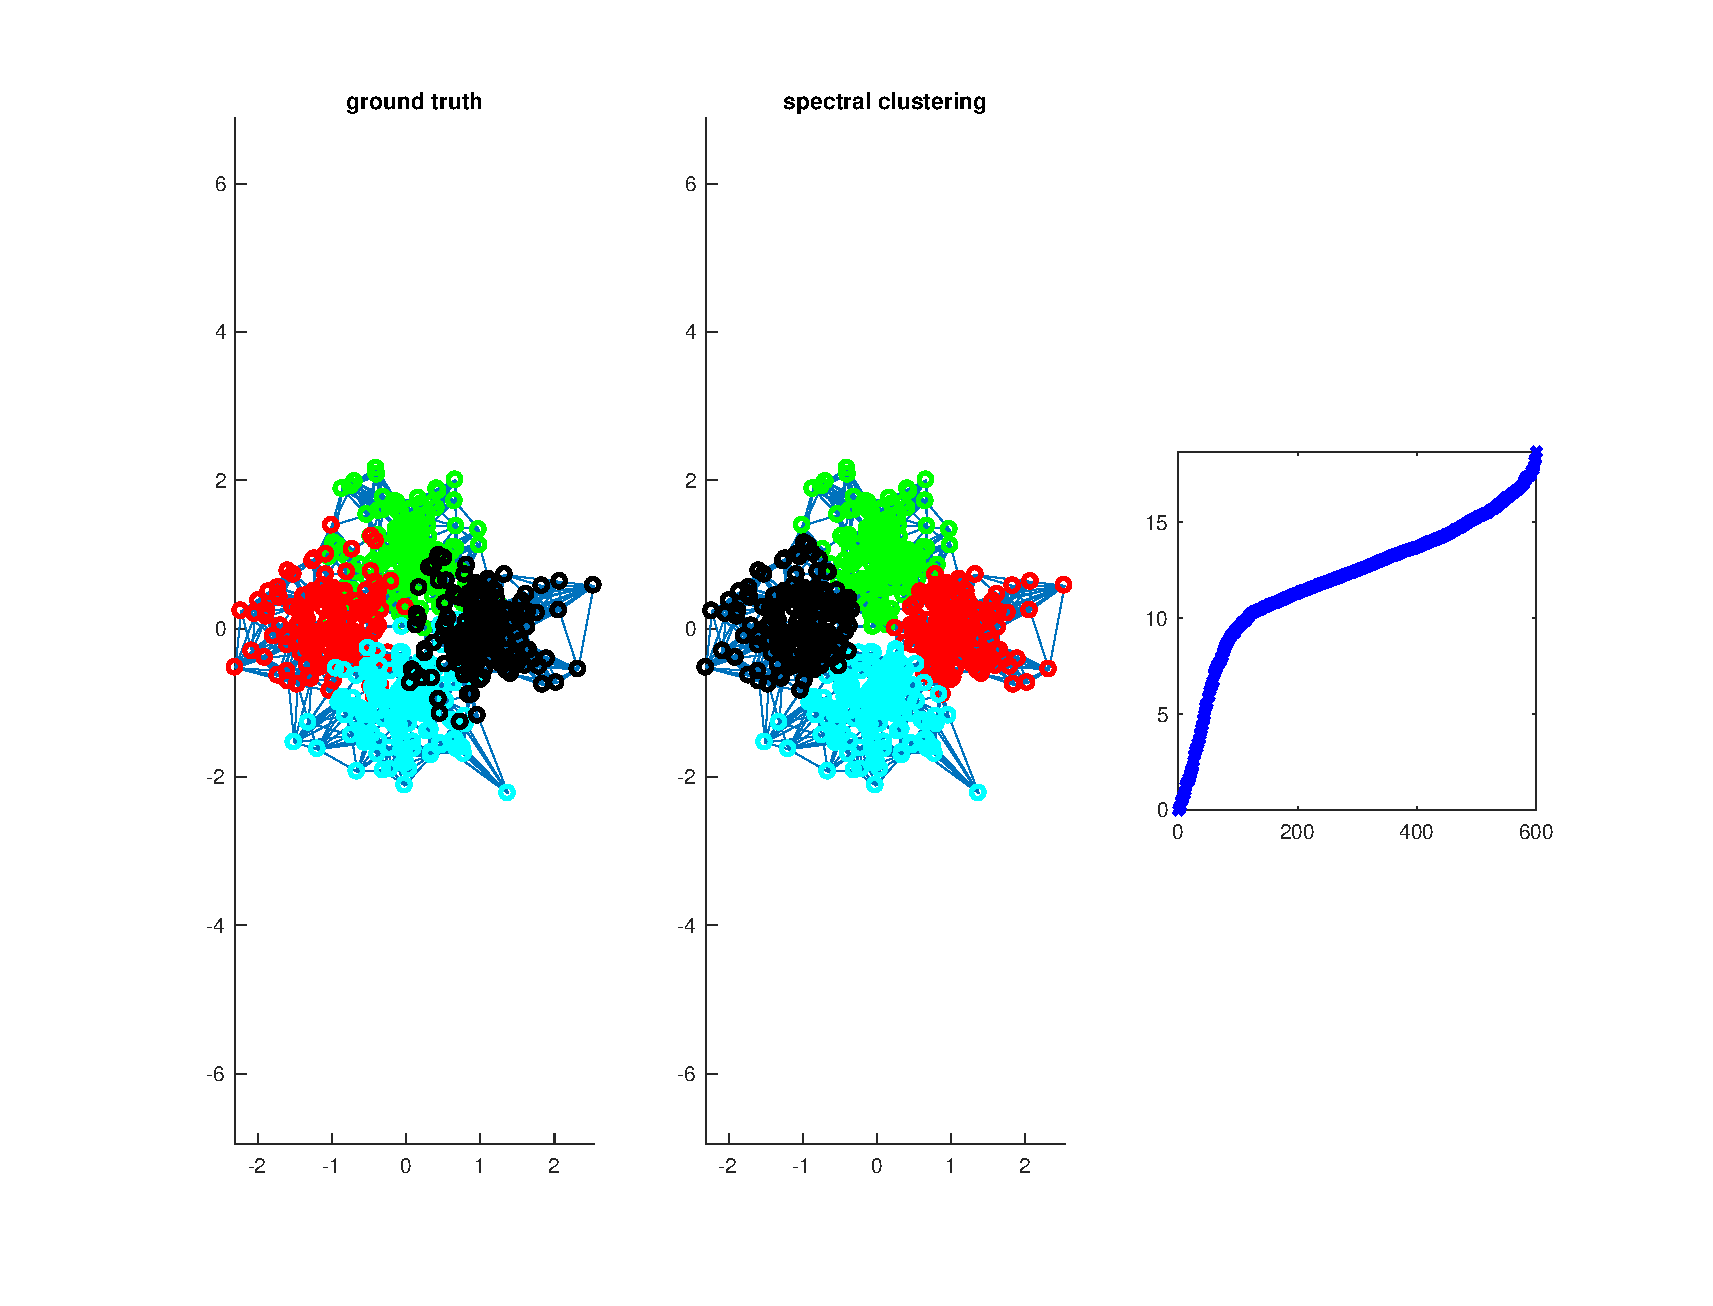
\includegraphics[width=13cm]{figures/two_blob_knn_0_20.eps}
\caption{Clustering with 4 blob and variance of 0.2}
\label{two_blob_knn_0_20}
\end{center}
\end{figure}

\question When you built the cluster assignment did you use thresholding, kmeans or both? Do you have any opinion on when to use each?
\begin{solution}
I used kmeans for the cluster assignment in the previous experiment and didn't try thresholding. However I think that kmeans allows to find more subtile clustering delimitation and consequently finer details of the data, however this method inherit from the instability of kmeans (due to its initialization...). On the other hand thresholding is more stable and would give more rectiligne, geometrical cluster delimitation.
\end{solution}


\question What is another use that looking at the distribution of the eigenvalues can have during clustering, beside choosing which eigenvectors to include?
\begin{solution}
Looking at the distribution of the eigenvalues can also help us to find how many cluster are lying in the dataset. Usually when doing clustering we don't know how many cluster we are looking for. If the graph is well constructed connected but not dense and not to sparse, the number of 'small" eigenvalue should reflect the number of cluster that structures our datasets.
\end{solution}

\question Plot your results using spectral clustering and k-means in two\_moons\_ clustering.m and compare the results. Do you notice any difference? Taking into consideration the graph structure, can you explain them?
\begin{solution}
For the two moons clustering, I used a $knn$ graph. I noticed that the results are very sensitive to number of neighbors used for building the graph. The best results are achieved with 7 nearest neighbors and are shown on the figure \ref{best_cluster_knn_7}. This number of neighbors allows to have only on connection between the two moons, where as in the others case either the graph is separated in two parts or there are many connections between the moons. Consequently it is much easer two cut the graph in the case where there is only one connection between to two heavily connected moons.
\end{solution}

\begin{figure}[!h]
\begin{center}
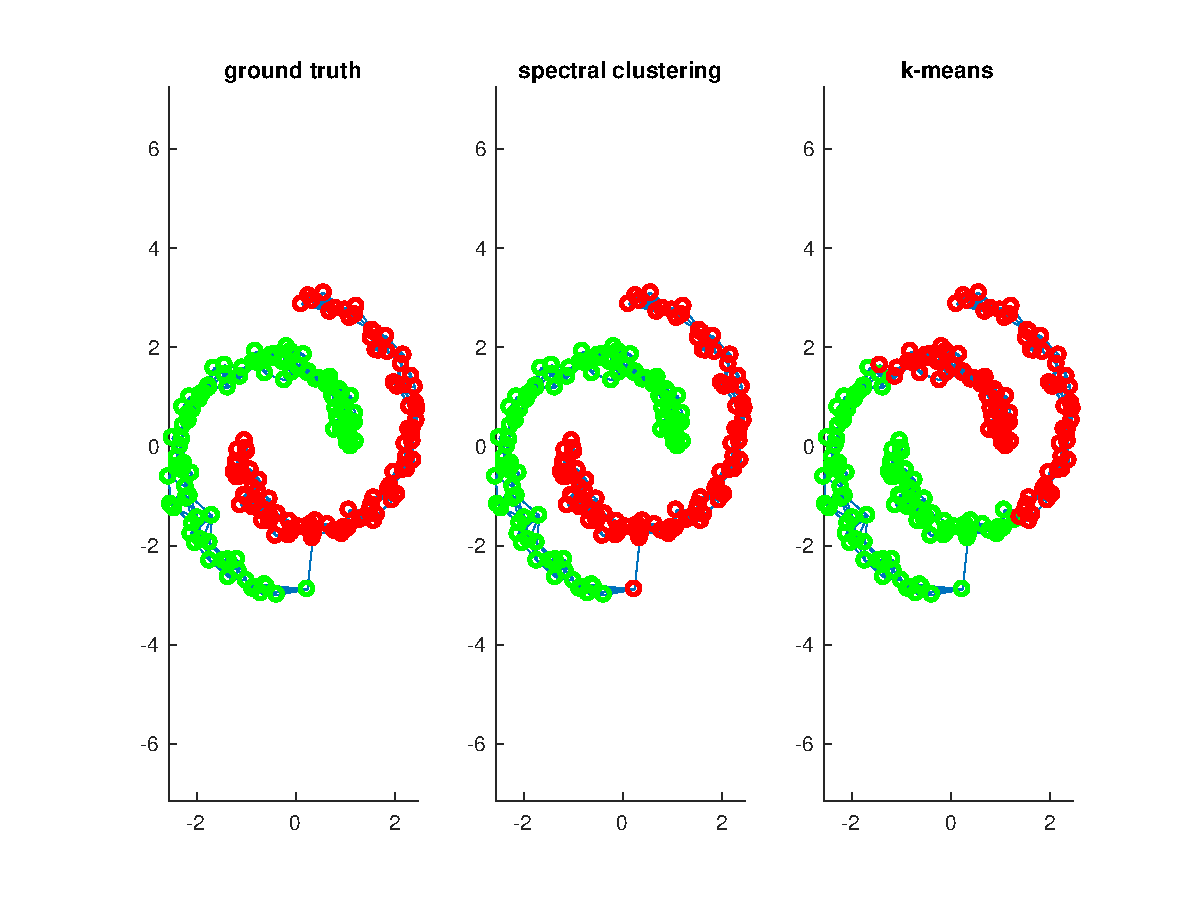
\includegraphics[width=13cm]{figures/best_cluster_knn_7.eps}
\caption{Clustering with 4 blob and variance of 0.2}
\label{best_cluster_knn_7}
\end{center}
\end{figure}

\question point\_and\_circle\_clustering.m will compare spectral clustering using the normal laplacian L and the random-walk regularized Laplacian Lrw. Do you notice any difference? Taking into consideration the graph structure, can you explain them?
\begin{solution}
Here we compare spectral clustering on the point and circle dataset for unnormalized and random-walk laplacian. We used a $knn-graph$ with 10 neighbors. We observe that using the normal laplacian doesn't manage to cluster the data whereas using the random-walk laplacian successfully cluster the dataset.\\

How to explain this effect ?\\
Unnormalized Laplacian solves the RatioCut (and MinCut) cutting strategy, whereas Normalized Laplacian solves the NCut strategy. The main difference between the two strategy is that NCut maximizes the Volume (sum of the weight in the cluster) of each cluster wheres RatioCut maximizes the cardinal of each cluster. If we look at the $point\_and\_circle$ dataset we have a very dense and close blob of point in the middle, a little gap and then around it a denser "ring" of points. If we want to cut the graph in two part, making a cut within the blob (or the ring) will penalize a lot the NCut object function because weight are high within the blob (or the ring) however it will less penalize the RatioCut because it won't impact the cardinality and on the other hand cutting the graph in between the blob and the ring is efficient for the NCut as the weight between the two group are much smaller. Consequently we can guess that in this case, the Normalized Laplacian has more chances at finding the right cluster than the Unnormalized Laplacian.

\end{solution}

\question Complete parameter\_sensitivity.m, and generate a plot of the ARI index while varying one of the parameters in the graph construction $\epsilon$ or k. Comment on the stability of spectral clustering.

\begin{figure}[!h]
\begin{center}
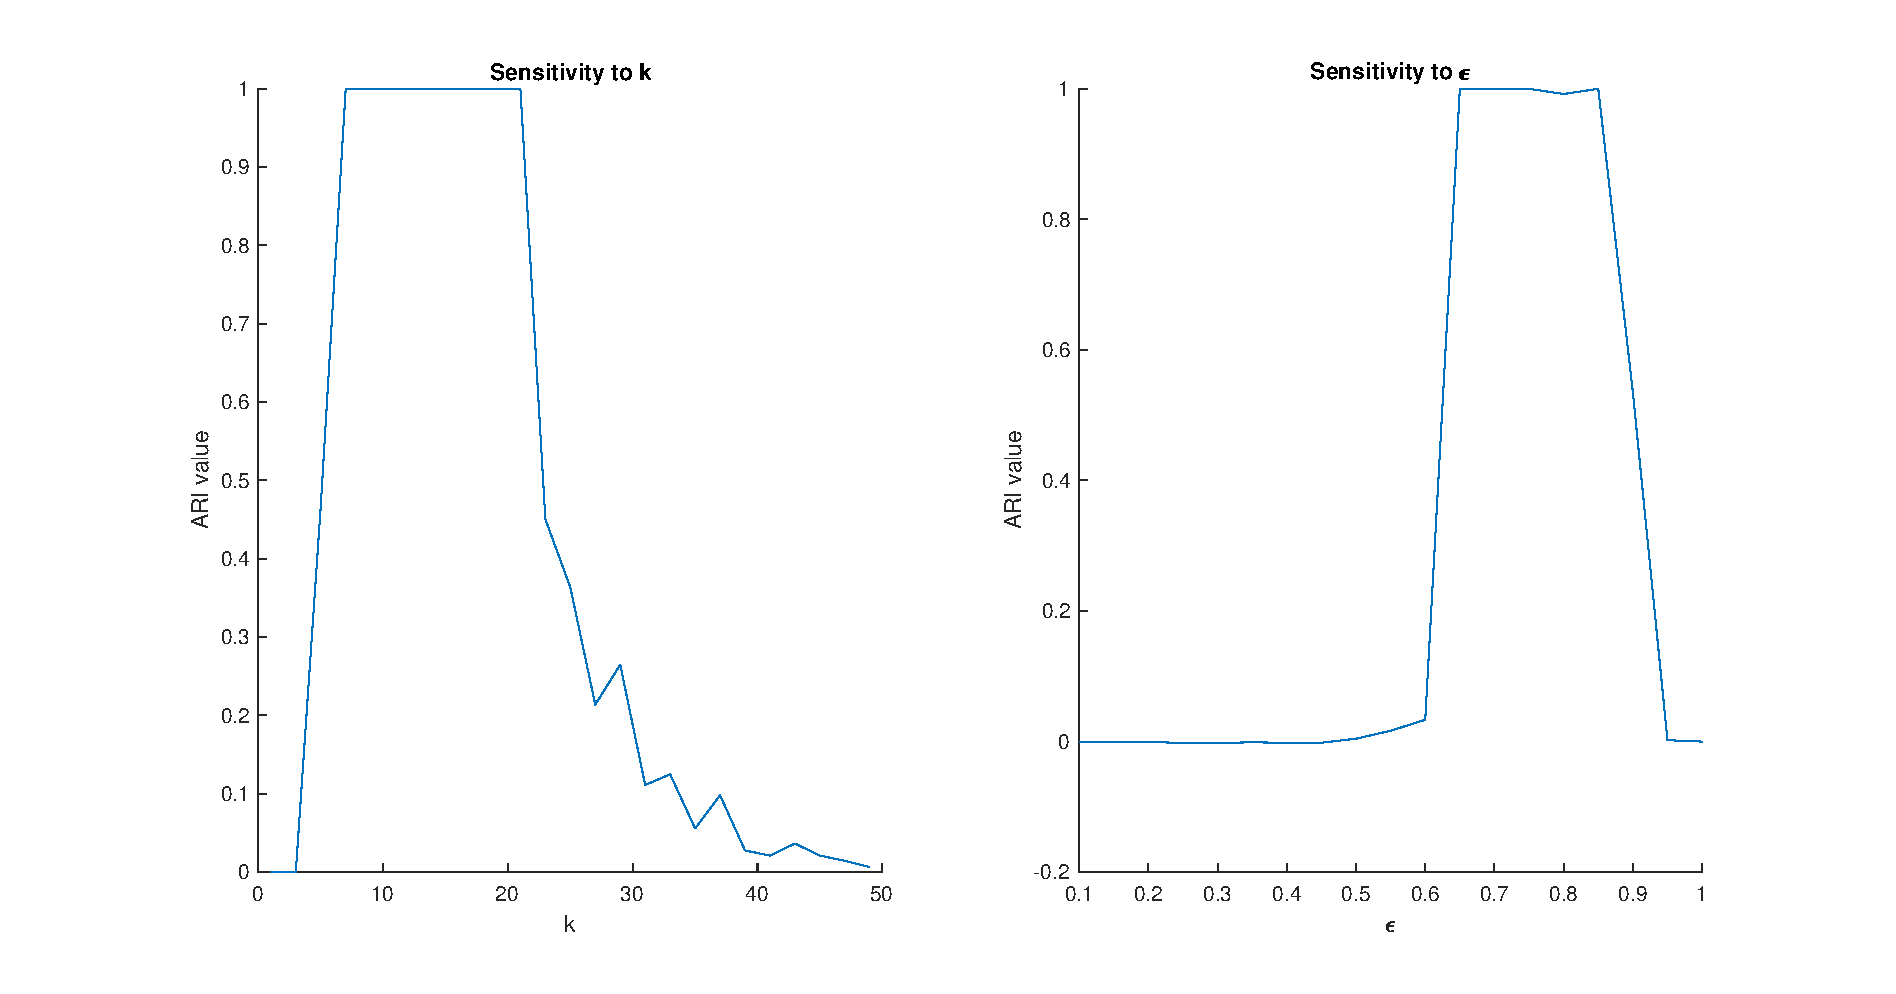
\includegraphics[width=13cm]{figures/compare_stability_k_eps.eps}
\caption{Comparing sensitivity of clustering to building parameter $k$ and $\epsilon$}
\label{compare_stability_k_eps}
\end{center}
\end{figure}

\begin{solution}
Sensitivity for each graph type ($\epsilon$ and $knn$) is plotted on figure \ref{compare_stability_k_eps}. We can see that for the two blob dataset that we use for this experiment, there are some "safe" interval: about [7,25] $k$ and about [0.7, 0.9] [$\epsilon$ that ensure some stability. This experiment was for blobs with low variance (0.02), if one tries to do it for higher variance (0.2 for instance), those curve are no longer true, and stability zone are much hard to find.
\end{solution}

\question If we did not have access to true1 labels how could we evaluate the clustering result (or what should we not use as evaluation)?
\begin{solution}
If no labels are available it is hard to evaluate clustering. One can't use ARI anymore, and using another clustering algorithm as a basis isn't a good idea to evaluate performance.
One way to sort or evaluate clustering result or at least compare several results, is to use the result of the clustering for another already tuned task which should be evaluable (for instance a supervised task) and compare this task results for different clustering.
\end{solution}

\end{questions}

%----------------------------------------------------------------------------------------
%	3. Image Segmentation
%----------------------------------------------------------------------------------------

\section{Image Segmentation}

\begin{questions}

\question The first documentation is the code. If your code is well written and well commented, that is enough. If you think you need to better express some of the choices you made in the implementation, you can use this question in the report. Remember to include all the related code in the submission
\begin{solution}
I would just add that I used for each part of the assignment a k\_main.m script (k = 1,2 or 3) that is the main script for reproducing the different results of questions.\\

Concerning the image segmentation part, I played a little bit with the graph parameter ($k$ and $\sigma$) to find a good couple : $k = 45$ and $\sigma = 5$. I also used my choose\_eig\_function to infer the number of cluster to use which I set also as the number of first eigenvector to use for clustering. Resuts for the two images are show on figure \ref{four_element_seg} and \ref {four_element_seg}
\end{solution}

\begin{figure}[!h]
\begin{center}
\includegraphics[width=13cm]{figures/fruit_salad_seg.jpg}
\caption{Image segmentation on the fruit\_salad image}
\label{fruit_salad_seg}
\end{center}
\end{figure}

\begin{figure}[!h]
\begin{center}
\includegraphics[width=13cm]{figures/four_element_seg.jpg}
\caption{Image segmentation on the four\_elements image}
\label{four_element_seg}
\end{center}
\end{figure}


\question A full graph built between the pixels of a 50 ? 50 image corresponds to 502 nodes. Solving the full eigenvalue problem in this case would scale in the order of 234. Even on weak hardware (i.e. iPhone) this takes only seconds to minutes. Segmenting a Full HD picture of 1920 ? 1080 would scale in the order of 264 (about a month on a decent machine i.e. not an iPhone). Beyond that, the large picture would require to store in memory a graph over millions of nodes. A full graph on that scale requires about 1TB of memory. Can you think two simple techniques to reduce the computational and occupational cost of Spectral Clustering?
\begin{solution}
To optimize the computational and occupational cost of spectral clustering there are two area of optimization : the similarity matrix (computation and storage) and finding the eigenvectors/values.
\begin{enumerate}
\item The literature suggest to use the Nystr�m approximation for finding eigenvalue without storing all the Laplacian. The method only relies on subsets of the Laplacian to  approximate its spectrum. However the downside is that this is only an approximation of eigenvalues/vectors.
\item Another solution is to quantize the laplacian is order to reduce the dimension, one could use clustering algorithm like $Kmeans$ to do so, or algorithm like the "Doubling algorithm", or graph embedding build using neural network.
\item To find the eigenvectors/values faster we used eigs instead of eig. see next question.
\end{enumerate}

\end{solution}

\question Did you use eig or eigs to extract the final eigenvectors? Shortly, what is the difference between the two? How do they scale to large graphs (order of complexity)?
\begin{solution}
I used eig but eigs in a much better choice for our application. Indeed it is much more efficient in our case as it only return the first n eigenvalue, which is what we want, we don't need all eigenvalue. Furthermore eigs is optimized for sparse matrix which is our case as the graph is not fully connected.\\
In terms of complexity,  $eig$ has a complexity of $\mathcal{O}(n^{3})$, but I don't know the complexity of $eigs$, it seems to vary with the sparsity of the matrix.
\end{solution}

\end{questions}


%----------------------------------------------------------------------------------------
%	BIBLIOGRAPHY
%----------------------------------------------------------------------------------------

\bibliographystyle{apalike}

\bibliography{sample}

%----------------------------------------------------------------------------------------


\end{document}